\cotefile{81}
\scanpage{27}
% archive sheet number: 26

cette dernière relation $\Sigma_1^-\cap\Sigma_2^-\ne\varnothing$ est vraie
$=$ si $E_1=E_2=\varnothing$, car
\deleted{\unsure{donc|alors} par hyp.} si on avait de plus
$\Sigma_1^-\cap\Sigma_2^-=\varnothing$, on en conclurait que les deux
\deleted{part.} décompositions binaires \deleted{\unsure{son|sont|se}}
(qui sont alors des partitions binaires) sont \uline{identiques},
ce que l'on \inserted{a} exclu. Cela montre que les
$\Sigma_1^+,\Sigma_2^+$ sont uniquement déterminés.

On a donc le diagramme d'inclusions
\diagram{\begin{tikzcd}[ampersand replacement=\&,column sep=small]
\Sigma_1^+ \& E_1 \arrow[l,hook] \arrow[r,hook] \& \Sigma_{12}
\& E_2 \arrow[l,hook] \arrow[r,hook] \& \Sigma_2^+
\end{tikzcd}}
qu'on, exprime par un diagramme
\figure{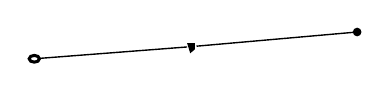
\begin{tikzpicture}[x=1cm,y=1cm]
\draw[line width=0.5pt] (0,0) -- (1.94,0.15);
\draw[line width=0.5pt] (2.06,0.16) -- (4.10,0.34);
\draw[fill=white,line width=1.1pt] (0,0) ellipse[x radius=0.065,y radius=0.043];
\fill (1.94,0.20) -- (2.04,0.20) -- (2.04,0.12) -- (1.98,0.07) -- cycle;
\fill (4.10,0.34) circle[radius=0.055];
\end{tikzpicture}}
\diagram{\begin{tikzcd}[ampersand replacement=\&,column sep=small]
\Sigma_1^+ \& E_1 \arrow[l,hook] \arrow[r,hook] \& \Sigma_{12}
\& E_2 \arrow[l,hook] \arrow[r,hook] \& \Sigma_2^+
\end{tikzcd}}

\margin{\[
\text{NB}\left\{\begin{aligned}
\Sigma_1^-&=\Sigma_{12}\amalg_{E_2}\Sigma_2^+\\
\Sigma_{\deleted{\unsure{1}}2}^-&=\deleted{E}\Sigma_{12}\amalg_{E_1}\Sigma_1^+
\end{aligned}\right.
\]}

% slanted
\margin{Ceci n'implique pas que les quatre ensembles
$\Sigma_1^+,\Sigma_1^-,\Sigma_2^+,\Sigma_2^-$ soient distincts,
car on peut avoir (\unsure{bien pas|non pas} $\Sigma_1^+=\Sigma_2^+$,
ni $\Sigma_1^-=\Sigma_2^-$, mais) $\Sigma_1^+=\Sigma_2^-$,
qui équivaut à $E_1=\Sigma_{12}$ et entraîne $E_2=\varnothing$
(\unsure{cela|Cela} signifie, en termes des $(\Sigma_{\unsure{1|t}}^+,\Sigma_1^-)$ que
$\Sigma_2^{\unsure{\dot{-}|-}}=\Sigma_1^+$,
$\Sigma_2^+=X\setminus\Sigma_1^+=\overset{\leftarrow}{\Sigma}{}_1^{-,\unsure{\circ|0}}$)
\deleted{\unsure{ou}} et la relation \unsure{symetrique|symétrique}.
On ne veut pas exclure ce cas, i.e.\ \deleted{\unsure{nous|mais}}
n'exige pas que les quatre ensembles
$\Sigma_1^+,\Sigma_1^-,\Sigma_2^+,\Sigma_2^-$ soient distincts
s'ils le \unsure{\deleted{sont}|sont}, on dit que les
\deleted{ens.} \inserted{deux décomp. bin.}
\deleted{\unsure{sont strictmt|sont strict.}} non parallèles.}

Je me propose d'étudier les ensembles finis
\unsure{indicellés|indiciellés}
$\deleted{\unsure{\Pi|\Sigma}}(\unsure{\Pi|\pi}_\alpha)_{\alpha\in A}
\deleted{=(\unsure{\Sigma_\alpha^i}),\unsure{\alpha\in A}}$
$\deleted{\Pi_\alpha=\{\Sigma_\alpha^\varepsilon}$
de décompositions binaires de $\unsure{X}$ deux à deux non parallèles.

Voici une façon très \unsure{générale|génerale}
d'\deleted{en}obtenir des \unsure{floppées|floppés}.

\scanpage{28}
Soit \unsure{.} $\Gamma=(S,A,R)$ un arbre ayant $S$ comme ens de sommets, $A$ \unsure{-} comme ens d'\unsure{aretes|arêtes}, $R$ comme \unsure{rèlation|rélation|relation} d'incidence [donc
$A\hookrightarrow\mathcal{P}_2(S)$, et $S\unsure{\hookrightarrow|\leftrightarrow|\mapsto}\mathcal{P}(A)$, et cette application est injective sauf si $\Gamma$ est isom au graphe
\diagram{\begin{tikzcd}[ampersand replacement=\&,column sep=1.4em]
\bullet \arrow[r,dash] \& \bullet
\end{tikzcd}}
]. Soi\deleted{t}ent $(U_s)_{s\in S}$ et $(E_a)_{a\in A}$ deux familles d'ensembles, et posons
\[
X=\coprod_{s\in S}U_s\ \amalg\ \coprod_{a\in A}E_a
\]

Pour tout $a_0\in A$, considérons les deux comp conn. $\deleted{\unsure{E}}\Gamma',\Gamma''$ de l'arbre $\Gamma$ ``coupé en $a_0$'', et \deleted{\unsure{c|con}}considérons la décomposition binaire . $X=X'\cup X''$ de $X$,
où
\[
\begin{aligned}
X'&=\coprod_{s\in S'}U_s\amalg\coprod_{a\in A'}E_a\\
X''&=\coprod_{s\in S''}U_s\amalg\deleted{\unsure{E}}\coprod_{\unsure{c|a}\in A''}E_a
\end{aligned}
\]
avec
\[
X'\cap X''=E_{a_0}
\]
cette décomposition est ``propre'' sss $\deleted{E}X'\ne E_{a_{\unsure{b|0}}},\ X''\ne E_{a_0}$. Ceci est le cas, quel que soit le choix de $a_0\in A$, sss on \unsure{a|à} la propriété \unsure{suivante|suivant} :

$(\unsure{\ast|A})$ Si $s\in S$ est un sommet-bout, alors $U_s\ne\varnothing$
% archive sheet number: 27

\scanpage{29}
% loc: upper-left slanted marginal note
\margin{$(\unsure{\ast\ast|\ast})$ \unsure{exprime|expriment|exprimons|exigeons} que si $a\ne b$, alors $\unsure{\Pi|\pi}_a\ne\Pi_b$}

% loc: opening paragraph and its interlinear/marginal replacement
De plus si $a_1,a_2\in A$, $a_1\ne a_2$, on voit de suite que les décompositions $\Pi_{a_1},\Pi_{a_2}$ sont bien parallèles, à cela près qu'il faut exiger \deleted{\unsure{que si $s$ est un sommet d'or}}%
\inserted{$(\ast\ast)$ si $s\in S$ est d'ordre $2$, alors un des trois ens $U_s,E_a,E_b$ est $\ne\varnothing$, où $a,b$ sont les deux arêtes inc. à $s$}

% loc: construction, including the annotation over the underlined gamma
Une \unsure{\deleted{façon}|façon} de visualiser la construction est via un arbre topologique $\deleted{A}\mathcal{X}=(\overset{\text{\inserted{esp. top.}}}{\underline{\Gamma}},S)$ (tel que $\Gamma$ en soit une description combinatoire). On fixe un pt sur chaque \unsure{arète|arête}, de façon à donner un graphe topologique (subdivision barycentrique) $\mathcal{X}^{\ast}=(\underline{\Gamma}^{\ast},\underbrace{S\amalg A'}_{S^{\ast}})$, où $A'\unsure{\in|\subset}\underline{\Gamma}$ est en corr \deleted{\unsure{b|bi}}biunivoque donnée avec \deleted{\unsure{tout}} $A$.

% loc: bracketed NB
\deleted{pt de} [\uline{NB} $A'$ est formé de \deleted{pts} sommets d'ordre $2$, et \inserted{pour} tte arête de $\unsure{\deleted{\underline{\Gamma}}}\mathcal{X}^{\ast}$, une exactement des deux extrémités appartient à $A'$, l'autre à $S$ -- voici une description complète des propriétés particulières aux $\underline{\Gamma}^{\ast}$\unsure{..|...}]

% loc: final paragraph; common letters remain live through the local corrections
Alors le\unsure{s|\deleted{s}} point\deleted{s} \inserted{$a'$} de $A'$ coupe\deleted{\unsure{nt}} $\underline{\Gamma}^{\deleted{\unsure{\ast}}}$ en deux composantes connexes, dont les adhérences définissent une décomposition binaire de $\underline{\Gamma}$, d'``équateur $\{a'\}$. Deux telles décompositions \deleted{bi} de $\underline{\Gamma}$, pour $a'\ne\unsure{a''|a'}$, définissent des décompositions binaires \unsure{str$^t$|stric$^t$|strict$^t$} non parallèles.
% archive sheet number: 28

\scanpage{30}
\unsure{Item|Idem|Itou}, si on regarde les traces de ces décompositions binaires sur $S^\ast=S\amalg A'$. Donc pour tte application \uline{surjective} $X\unsure{\mathrel{\text{---}}|\longrightarrow}S^\ast$, si on regarde les des images inverses des décompositions binaires précédentes de $S^\ast$. \unsure{\deleted{D}}Or la donnée d'une telle application, revient à celle d'une famille $(X_\sigma)_{\sigma\in S^{\unsure{\ast|+}}}$ \inserted{d'ens $\ne\varnothing$}, i.e. \deleted{à} celle des deux familles $(U_s)_{s\in S}$ et $(E_a)_{a\in A}$ d'ens non vides.

Le cas où certains des ensembles $U_s,E_a$ pourraient être vides est à examiner avec plus de soin, il donne néanmoins ce qu'on veut sss on a les conditions $(\ast)$ $(\ast\ast)$ ci-dessus, et la condition de non-parallélisme stricte sss on a \uline{ceci} (plus fort que $(\ast\ast)$)

$(\ast\ast\ast)$ Si $s\in S$ est un sommet \uline{d'ordre 2} \deleted{tel} \inserted{et} \deleted{que $U_s=\varnothing$, et} \inserted{$a\in A$ une arête incidente, on a}
\[
U_s\ne\varnothing\ \unsure{\text{ou}|\text{--}}\ E_{\unsure{c|a}}\ne\varnothing
\]
% archive sheet number: 29

\scanpage{32}
% archive sheet number: 31
\begingroup
\makeatletter\tagsleft@true\makeatother

\margin{\uline{Version II}}
\noindent Décompositions $n$-aires d'un espace topologique\unsure{.}

1.1. Soit $X$ un espace topologique. On appelle \uline{décomposition binaire} de $X$ une paire (\unsure{notée|noté} indiciellement)
\[
\unsure{\pi|\Pi}=(\Sigma^\varepsilon)_{\varepsilon\in\omega}\qquad(\omega\ \text{ens \unsure{:|à} deux éléments})
\]
\unsure{dé|de|d'e} \deleted{ensembles} parties \uline{fermées} (distinctes) de $X$, de réunion $X$
\[
X=\bigcup_{\varepsilon\in\omega}\Sigma^\varepsilon.\tag*{(1)}
\]

On suppose que
\[
\Sigma^\varepsilon\ne\varnothing\qquad(\forall\varepsilon\in\omega)\tag*{(2)}
\]
ce qui signifie aussi que
\[
\pi\ne\{\varnothing,X\}\tag*{$(2')$}
\]
et implique que $X\ne\varnothing$, et même $\mathrm{card}\,X\geq 2$, puisque l'on a supposé
\[
\unsure{\deleted{X|\Sigma}}\Sigma^\varepsilon\unsure{\deleted{=|\ne}}\ne\Sigma^{\varepsilon'}\qquad\text{si }\varepsilon,\varepsilon'\in\omega,\quad\varepsilon\ne\varepsilon'.\tag*{(\unsure{3|s|$\wedge$})}
\]

On n'exclut pas le cas où on aurait une inclusion
\[
\Sigma^{\varepsilon'}\subset\Sigma^\varepsilon
\]
ce qui équivaut, par (1), à la relation
\[
\Sigma^\varepsilon=X.
\]

Les $\Sigma^\varepsilon$ $(\varepsilon\in\omega)$ s'appellent les \uline{\unsure{hémisphéres|hémisphères}} de la décomposition binaire, \deleted{la} et l'ensemble
\[
E=\bigcap_{\deleted{\omega}\varepsilon\in\omega}\Sigma^\omega\tag*{(4)}
\]
s'appelle l'\uline{équateur} de la décomposition binaire.

On n'exclut pas le cas où on aurait $E=\varnothing$, ce qui indique que les $\Sigma^\varepsilon$ \inserted{$(\varepsilon\in\omega)$} sont \inserted{complémentaires l'un de l'autre, \unsure{donc}} à la fois fermés et ouverts -- donc que $X$ est disconnexe.
\endgroup

\scanpage{33}
% archive sheet number: 32
\begingroup
\makeatletter\tagsleft@true\makeatother
Notons les implications
\[
\left\{\begin{aligned}
&X\ \text{connexe}\quad\Longrightarrow\quad E\overset{\mathrm{def}}{=}\bigcap_{\varepsilon\in\omega}\deleted{\unsure{X|\Sigma}}\Sigma^\varepsilon\ \unsure{-|\deleted{-}}\unsure{\deleted{=|\varnothing}}\ne\varnothing\\
&\text{Si les }\Sigma^\varepsilon\ \text{connexes, alors}\quad X\ \text{connexe}\ \Longleftrightarrow\ E\ne\varnothing.
\end{aligned}\right.\tag*{\shortstack[l]{(5)\\\unsure{,|'}}}
\]

Nous poserons
\[
\Sigma^{\unsure{\circ|o|0}\varepsilon}=\Sigma^\varepsilon\setminus E=\Sigma^\varepsilon\setminus\Sigma^\varepsilon\cap\Sigma^{\varepsilon'}=X\setminus\Sigma^{\varepsilon'}\qquad(\omega\unsure{\in|\ne|=}\{\varepsilon,\varepsilon'\})\tag*{(6)}
\]
de sorte que l'on a la décomposition
\[
X=\Sigma^{\circ\unsure{\deleted{2|\varepsilon}}\varepsilon_{\unsure{\deleted{1|+}}.}}\cup E\cup\Sigma^{\circ\varepsilon'_{\unsure{\deleted{2|-}}}}\qquad(\omega=\{\varepsilon'_{\unsure{\deleted{1|+}}},\varepsilon'_{\unsure{\deleted{2|-}}}\})\tag*{(7)}
\]
de $X$ en \deleted{trois} ens. mutuellement disjoints.

Notons
\[
\overline{\Sigma^{\circ\varepsilon}}\cap E=\overline{\Sigma^{\circ\varepsilon}}\cap\Sigma^{\varepsilon'}=\overline{\Sigma^{\circ\varepsilon}}\setminus\Sigma^{\circ\varepsilon}=\dot{\Sigma}^{\circ,\varepsilon}\quad\unsure{\varepsilon,|;|\varepsilon|,}\tag*{(8)}
\]

\deleted{On a le cas}\par
\deleted{on s'intéresse à la cond}

1.2. Deux décompositions binaires
\[
\unsure{\pi|\Pi}_1=\{\Sigma_{\deleted{\unsure{\varepsilon|2}}1}^\varepsilon\}_{\varepsilon\in\omega_1},\qquad\pi_2=\{\Sigma_2^\varepsilon\}_{\varepsilon\in\omega_2}\tag*{(9)}
\]
sont dites non \uline{\unsure{parallèles|paralèles}}, \inserted{si elles sont distinctes, et} s'il existe un . $\Sigma_1^+\in\pi_1$, et un $\Sigma_2^+\in\pi_2$, tels que l'on ait
\[
\Sigma_1^+\cap\Sigma_2^+=\varnothing\tag*{(10)}
\]
condition qui équivaut \unsure{:|à}
\[
\Sigma_1^+\subset\Sigma_2^-\tag*{(11)}
\]
ou encore :
\[
\Sigma_2^+\subset\Sigma_1^-\tag*{(\unsure{11'bis|11bis|11 bis})}
\]
où $\Sigma_1^-,\Sigma_{\unsure{2|1}}^-$ sont definis par
\[
\pi_1=\{\Sigma_1^+,\Sigma_1^-\},\qquad\pi_2=\{\Sigma_2^+,\Sigma_{\unsure{2|1}}^-\}\tag*{(\unsure{17|12})}
\]
\endgroup

\scanpage{34}
% archive sheet number: 33
\begingroup
\makeatletter\tagsleft@true\makeatother
Posons
\[
\Sigma_{12}=\Sigma_1^-\cap\Sigma_2^-,\qquad E_1=\Sigma_1^+\cap\Sigma_1^-,\quad E_2=\Sigma_1^+\cap\Sigma_2^-\tag*{(13)}
\]
alors on a le diagramme d'inclusion de parties fermées de $X$
\usetikzlibrary{decorations.pathmorphing}
\diagram{\[
\begin{tikzcd}[ampersand replacement=\&,row sep=1.1em,column sep=.4em]
\& \& X \& \& \\
\& \Sigma_2^- \arrow[ur] \& \& \Sigma_1^- \arrow[ul] \& \\
\Sigma_1^+ \arrow[ur] \& \& \Sigma_{12} \arrow[ul]\arrow[ur] \& \& \Sigma_2^+ \arrow[ul]\\
\& E_1 \arrow[ul]\arrow[ur] \& \& E_2 \arrow[ul]\arrow[ur] \& \\
\& \& \unsure{\deleted{\Omega}|\Omega|\deleted{2}|\deleted{\varnothing}}\arrow[ul]\arrow[ul,no head,decorate,decoration={zigzag,segment length=3.4pt,amplitude=1.6pt}] \& \&
\end{tikzcd}\tag*{(14)}
\]}
\margin{NB $\Sigma_1^+\cap\Sigma_2^+=\varnothing$ \unsure{donc|donne} $E_1\cap\Sigma_2^+=\varnothing$, $E_2\cap\Sigma_1^-=\varnothing$ i.e. $E_1\subset\Sigma_2^{\unsure{\circ|o|0}-}$, $E_2\subset\Sigma_1^{\circ-}$ et $E_1\cap E_2\unsure{-|.}=\varnothing$}
où \unsure{les|le} trois carrés sont cartésiens et cocartésiens
\[
\deleted{E_1}
\]
i.e.
\[
\left|\begin{aligned}
&E_1=\Sigma_1^+\cap\Sigma_{12},\quad\Sigma_2^-=\Sigma_1^+\cup\Sigma_{12}\\
&\deleted{\unsure{E_1|E}}
\end{aligned}\right.
\]
et les deux relations analogues correspondant aux deux autres carrés
\[
\left\{\begin{aligned}
&E_2=\Sigma_{\unsure{\deleted{2|1}}12}^{\deleted{\unsure{+|-}}}\cap\Sigma_{\deleted{\unsure{12|1}}2}^+,\quad \Sigma_1^-=\Sigma_{22}^{\deleted{\unsure{+|-}}}\cup\Sigma_2^+\\
&\Sigma_{12}\overset{(13)}{\equiv}\Sigma_1^-\cap\Sigma_{\unsure{2|1}}^-,\quad \unsure{\deleted{{-}|\Sigma}}X=\Sigma_2^-\cup\Sigma_1^-.
\end{aligned}\right.\tag*{(15)}
\]
Notons que
\[
\left\{\begin{aligned}
&\text{a)}\quad\Sigma_1^+\cap\Sigma_2^-=\Sigma_1^+\ne\varnothing\\
&\text{b)}\quad\Sigma_2^+\cap\Sigma_1^-=\Sigma_2^+\ne\varnothing\\
&\text{c)}\quad\Sigma_1^-\cap\Sigma_2^-=\Sigma_{12}\ne\varnothing,
\end{aligned}\right.\tag*{(16)}
\]
\inserted{\unsure{Prouvons|Prenons}} \unsure{La|la} \unsure{derniêre|dernière} relation (les deux premières étant évidentes).
Si on a\unsure{\deleted{vait}|vait|\deleted{ura}} $\Sigma_{12}=\varnothing$, comme $E_1,E_2\subset\Sigma_{12}$, on aurait $E_1=\varnothing$, $E_2=\varnothing$, de sorte que $\unsure{\Pi|\pi}_1$ et $\Pi_2$ sont deux \uline{partitions} de $X$ en des parties non vides, i.e. $\deleted{\Sigma_{\unsure{1|2}}^- = X\setminus{\unsure{{-}|\Sigma}}^-}$ on \unsure{aurait|avait}
\[
\deleted{\Sigma_1^+}\quad\Sigma_1^-=X\setminus\Sigma_1^+,\quad\Sigma_2^-=X\setminus\Sigma_2^+
\]
\endgroup

\scanpage{35}
d'où
\[
\Sigma_{12}=X\deleted{-}\setminus(\Sigma_1^+\cup\Sigma_2^+)
\]
\unsure{donc} $\Sigma_{12}=\varnothing$ signifierait que
\[
X=\Sigma_1^+\amalg\Sigma_2^+
\]
et par suite
\[
\unsure{\Pi|\pi}_1=\left\{\Sigma_1^+,\underset{\inserted{\substack{\Vert\\\Sigma_{\unsure{\deleted{2|1}}\unsure{1|2}}^-=\unsure{\deleted{{-}|\Sigma}}X\unsure{\deleted{-}}\setminus\Sigma_1^+}}}{\Sigma_2^+}\right\},
\qquad\Pi_2=\{\Sigma_2^+,\Sigma_1^+\}
\]
alors $\deleted{\unsure{\Pi_2|\Pi_1}}\quad\Pi_1=\Pi_3$ contrairement : l'\unsure{hypothèse|hypothese}.

On trouve donc

\noindent\deleted{\uline{Corollaire}} \inserted{Proposition} \unsure{Soient|Soit} $\Pi_1;\unsure{\deleted{\vert}}\Pi_2$ deux décompositions\\
\makebox[0pt][r]{\rule[-2.7ex]{.4pt}{3.8ex}\hspace{.45em}}binaires de $X$, mutuellement non panachées.\\
Alors il existe un \uline{unique} couple
\[
(\Sigma_1^{\unsure{\top|+}},\Sigma_2^+)\in\Pi_1\times\Pi_2
\]
\noindent\makebox[0pt][r]{\rule[-.35ex]{.4pt}{2ex}\hspace{.45em}}tel que l'on ait
\[
\Sigma_1^+\cap\Sigma_2^+=\varnothing
\]

\begingroup\makeatletter\tagsleft@true\makeatother
Soit alors
\[
C=\Pi_1\amalg\Pi_2=\omega_1\amalg\omega_2
\tag*{(17)}
\]
l'ensemble somme, qui a quatre éléments. On a une application canonique
\[
C\longrightarrow{\unsure{\mathfrak{P}|\mathcal{P}}}_{\unsure{\text{finies}|\text{fermés}|\text{fermé}}}(X)
\tag*{(1\deleted{7}8)}
\]
qui a comme image
\[
\{\Sigma_1^+,\Sigma_1^-,\Sigma_2^+,\Sigma_2^-\},
\tag*{(1\deleted{8}9)}
\]
et laquelle on l'identifie si $(1\deleted{\unsure{7}}8)$ est injective, i.e.
\endgroup
\clearpage
% archive sheet number: 34

\scanpage{36}
% archive sheet number: 35
\begingroup\makeatletter\tagsleft@true\makeatother
si \deleted{\unsure{Card|le}} cardinal de l'ens. $(18)$ est $4$, i.e. si les quatre parties de $X$
\[
\Sigma_1^+,\quad\Sigma_1^-,\quad\Sigma_2^+,\quad\Sigma_2^-
\]
sont distinctes. A ce propos notons que l'on sait déjà par \deleted{hypothèse $(\unsure{\Pi|\pi}_1,\Pi_2$ \unsure{étant}} \inserted{définition} des déc. binaires
\[
\Sigma_1^+\ne\Sigma_1^-,\qquad\Sigma_2^+\ne\Sigma_2^-
\tag*{($*$)}
\]
et qu'on a
\[
\Sigma_1^+\ne\Sigma_2^+
\tag*{($**$)}
\]
puisque $\Sigma_1^+$ et $\unsure{\Sigma|\Sigma_2}^{\unsure{+|\top}}$ sont des parties disjointes \uline{non} \uline{vides}. Notons donc qu'on lit sur le diagramme $(14)$
\[
\left\{\begin{aligned}
\text{a)}\;(\Sigma_1^+\unsure{\ne|=}\Sigma_2^-)&\Longleftrightarrow E_1\unsure{\ne|=}\Sigma_{12}
   &(\Longrightarrow E_2=\varnothing)\\
\text{b)}\;(\Sigma_2^+=\Sigma_1^-)&\unsure{\Longleftrightarrow|\Longrightarrow} E_2=\Sigma_{12}
   &(\Longrightarrow E_1=\varnothing)
\end{aligned}\right.
\tag*{($***$)}
\]
et que les deux relations \inserted{\unsure{-|a}), b)} envisagées dans $(***)$ ne peuvent être satisfaites simultanément, puisque $\deleted{\Sigma_{12}}$ l'on aurait $\Sigma_{12}=E_1=E_2=\varnothing$ puisque $E_1\cap E_2=\varnothing$, ce qui contredit $(16)$ (c).

Enfin
\[
(\Sigma_1^-=\Sigma_2^-)\Longleftrightarrow
(\Sigma_{1\unsure{\deleted{2}|2}}^-=\unsure{\deleted{X|E}}\Sigma_2^-=X)
\quad\text{i.e. }\Sigma_{12}=X
\tag*{($****$)}
\]
Ce cas est mutuellement exclusif avec chacun des cas $(***)$, \deleted{\unsure{dans ces derniers}} \inserted{\unsure{Car|car} si on avait en $=$ temps} $\deleted{\unsure{\Sigma_1^-}=\Sigma_2^-=X}\ \unsure{\deleted{E}}\Sigma_{12}=X$ et $E_1=\Sigma_{12}$, on aurait $E_1=X$ donc $\Sigma_1^+=\Sigma_1^-=X$, \deleted{\unsure{de|et}}\unsure{ce} qui contredit $(3)$.

\uline{Proposition} Pour que l'on ait $\operatorname{Card}\{\Sigma_1^+,\Sigma_1^-,\Sigma_2^+,\Sigma_{\unsure{2|1}}^-\}=4$, il faut et il suffit que l'on ne soit pas l'un des trois cas suivants, qui s'excluent mutuellement
\[
\left\{\begin{aligned}
\text{\unsure{a})}\quad &E_1=\Sigma_{12}&&(\Longrightarrow E_2=\varnothing)\\
\text{a')}\quad &E_2=\Sigma_{12}&&(\Longrightarrow E_1=\varnothing)\\
\text{b)}\quad &\Sigma_{12}=X\quad\text{i.e. }\Sigma_1^-=\Sigma_2^-=X
   &&(\text{d'où }E_1=\Sigma_1^+,E_2=\Sigma_2^+)
\end{aligned}\right.
\tag*{(\deleted{\unsure{19|20}}20)}
\]
auquel cas le cardinal \unsure{du|des|de} $\unsure{\}\,4|\{\ \}|4}$ est égal \unsure{:|à} \unsure{trois}.

\endgroup
\clearpage

\scanpage{37}
% archive sheet number: 36
\begingroup\makeatletter\tagsleft@true\makeatother
\uline{Cor} \deleted{D}ans le cas où $\operatorname{Card}\{\ \}=4$, \inserted{et $\Sigma_1^-\ne X,\Sigma_2^-\ne X$} les seules relations d'inclusions entre les ensembles $\Sigma_1^+,\Sigma_1^-,\Sigma_2^+,\Sigma_2^-$ sont les relations
\margin{Sous forme : Pour que les relations \unsure{strictes} $(*)$ soient les seules relations d'inclusion entre les ensembles $\Sigma_1^+,\Sigma_1^-,\Sigma_2^+,\Sigma_{\unsure{1|2}}^-$, il f et s. que ceux-ci soient \inserted{\unsure{mutlt.|mult.}} distincts et que l'on ait $\Sigma_1^-\ne X,\Sigma_2^-\ne X$.}
\[
\left\{\begin{aligned}
\Sigma_1^{\unsure{\top|+}}&\subset\Sigma_2^-\\
\Sigma_2^+&\subset\Sigma_1^-
\end{aligned}\right.\qquad .
\tag*{($*$)}
\]
En effet, on n'a pas les inclusions inverses, par hypothèse. D'autre part, on n'\uline{a pas}
\[
\Sigma_1^+\subset\Sigma_1^-\quad\text{ou}\quad
\Sigma_1^-\unsure{\subset|\in}\Sigma_1^+,\quad\text{car on aurait}
\]
$\deleted{\Sigma_1^+,\unsure{\Sigma_1|\Sigma_1^+|\Sigma_1^-}}\ \Sigma_1^-=X$, de $=$ on n'a pas $\Sigma_2^+\subset\unsure{\deleted{\vert}}{\unsure{\Sigma|E}}_{\unsure{1|2}}^-$ ni $\Sigma_2^-\subset\Sigma_2^+$, et on n'a pas $\Sigma_1^+\subset\Sigma_2^+$ ni l'inclusion inverse, puisque $\Sigma_1^+$ et $\unsure{\Sigma|\Sigma_2}^{\top}$ sont disjoints et $\ne\varnothing$. Il reste à voir que l'on n'a pas une inclusion $\Sigma_1^-\subset\Sigma_2^-$ ou inclusion inverse, on lit sur le diagramme $(14)$ que \deleted{\unsure{cela}} \inserted{la première \unsure{p.ex.|p. ex.}} signifierait que $\deleted{\Sigma_{12}\simeq\Sigma_1^-}$ \deleted{\unsure{d'où|de}} $\Sigma_2^-=X$, ce que l'on a exclu.

% The two thin, slightly wavering segments below reproduce the left marginal rule.
\noindent\begin{minipage}[t]{.04\linewidth}
\vspace{1.2\baselineskip}
\figure{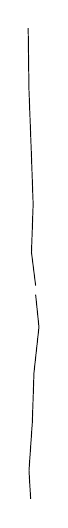
\begin{tikzpicture}[x=.3pt,y=.3pt]
\draw[line width=.35pt] (0,0) -- (1,-75) -- (4,-155) -- (6,-212) -- (4,-270) -- (9,-310);
\draw[line width=.35pt] (9,-321) -- (13,-360) -- (7,-415) -- (5,-475) -- (1,-533) -- (3,-567);
\end{tikzpicture}}
\end{minipage}\hfill\begin{minipage}[t]{.94\linewidth}
\vspace{0pt}
\uline{\unsure{Dêf|Déf}} On dit que $\unsure{\Pi|\pi}_1,\unsure{\Pi|R}_2$ sont \uline{\unsure{strictement|Strictement} non\unsure{:|.} panachées} \inserted{si elles sont non panachées, et} si l\unsure{\deleted{es}}es quatre ensembles $\Sigma_1^\top,\Sigma_1^-,\Sigma_2^+,\Sigma_2^-$ sont distincts, \unsure{et.|i.e.} si \unsure{((|c} de plus $\Sigma_1^-\ne X,\Sigma_2^-\ne X$ -- i.e si les seules relations d'inclusion entre les ensembles $\Sigma_1^\top,\Sigma_1^-,\Sigma_2^\top,\Sigma_2^-$ sont $\Sigma_1^+\subset\Sigma_2^-,\Sigma_2^+\subset\Sigma_1^-$ -- ce qui signifie aussi que l'on a :
\[
\Sigma_1^-\ne X,\Sigma_2^-\ne X
\quad(\text{on dit donc que }\Pi_{\unsure{1|2}},\Pi_2\text{ sont \uline{propres}}),
\ E_1\ne\Sigma_{12},E_2\ne\Sigma_{12}.
\tag*{(21)}
\]
\end{minipage}
\endgroup
\clearpage

\scanpage{38}
\begingroup\makeatletter\tagsleft@true\makeatother
Mais si cette condition n'est pas satisfaite pour $\unsure{\deleted{\Sigma|E}}\unsure{\Pi|\pi}_1,\Pi_2$ non panachées, on reste en plan, et on regarde l'ens. \unsure{:|à} quatre éléments
\[
C=\Pi_1\amalg\Pi_2=\omega_1\amalg\omega_2
=\{\varepsilon_1^{\unsure{\top|+}},\varepsilon_1^-,\varepsilon_2^{\top},\varepsilon_2^-\}
\tag*{(17)}
\]
et la relation d'ordre dessus, \unsure{ou|où} les seules relations $<$ sont données par
\[
\varepsilon_1^+<\varepsilon_2^-,\qquad\varepsilon_2^+<\varepsilon_1^-
\tag*{(22)}
\]
\diagram{\begin{tikzcd}[ampersand replacement=\&,row sep=2.3em,column sep=2.6em]
|[label=left:{\(\varepsilon_1^-\)}]| \bullet \arrow[from=2-2,to=1-1]
 \& |[label=right:{\(\varepsilon_2^-\)}]| \bullet\\
|[label=left:{\(\varepsilon_1^+\)},label=below:{\(\deleted{\unsure{\varepsilon_2^+|\varepsilon_1^+}}\)}]| \bullet \arrow[ur,crossing over]
 \& |[label=right:{\(\varepsilon_2^+\)}]| \bullet
\end{tikzcd}}

1.3. Soit \deleted{$(\Pi_\alpha)_{\alpha\in A}$ une famille}
\[
(\Pi_\alpha)_{\alpha\in A},\qquad \Pi_\alpha=\{\Sigma_\alpha^\varepsilon\}_{\varepsilon\in\omega_\alpha}
\tag*{(23)}
\]
% slanted in the left margin, beside (23)
\margin{c'est un élément de $\unsure{\mathfrak{P}|\mathcal{P}}(\mathfrak{P}_2(\unsure{\deleted{X|\times}}\unsure{\mathfrak{P}|\mathcal{P}|\square})(X))$}
\unsure{une|un} \deleted{famille} \inserted{ens. (\unsure{écrit|écrite|noté} \unsure{indiciellement|individuellement})} de décompositions binaires de $X$, on suppose \deleted{qu'elles}
\[
\forall\alpha,\beta\in A,\quad\alpha\ne\beta,\qquad
\Pi_\alpha,\Pi_\beta\ \text{sont \unsure{mut|mul}\textsuperscript{t}. non panachées\unsure{.}}
\tag*{(24)}
\]
% slanted in the left margin, beside (24) and the definition
\margin{On dit, si $\operatorname{Card} A=\unsure{n|\nu}$, que l'on a une \uline{décomposition} \uline{$n$-aire} non panachée de $X$}

\inserted{\uline{\unsure{D\.ef|Déf}}} On dit \deleted{alors} que $(\Pi_\alpha)_{\alpha\in A}$ est non \unsure{panachée|panachées}. (Terminologie analogue pour \uline{strictement} non panachée).

Considérons
\[
C=\coprod_{\alpha\in A}\omega_\alpha
\tag*{(25)}
\]
\inserted{avec l'involution ss p\textsuperscript{t} fixe $\sigma$ qui, sur chaque $\omega_\alpha$, induit une \deleted{\illegible{1}} transposition}
et sur $C$ la relation d'ordre, dans laquelle on a

\endgroup
\clearpage
% archive sheet number: 37

\scanpage{39}
\begingroup\makeatletter\tagsleft@true\makeatother
\[
\left(
\underset{\substack{\rotatebox{-90}{$\in$}\\\omega_\alpha}}{x}
<
\underset{\substack{\rotatebox{-90}{$\in$}\\\omega_\beta}}{y}
\right)
\Longleftrightarrow
\Biggl(\alpha\ne\beta,\quad
\underbrace{x\underset{\{\unsure{\Pi|\pi}_\alpha,\Pi_\beta\}}{<}y}_{
\inserted{\substack{\text{i.e. }\deleted{\unsure{x}}\\
\Sigma_\alpha^x\cap\Sigma_\beta^{\sigma y}=\varnothing}}}
\Biggr)
\tag*{(26)}
\]
\margin{il faut vérifier la \unsure{transitivité} de cette relation -- c'est \unsure{immédiat}}

Alors $\sigma$ est un antiautomorphisme (involutif sans p\textsuperscript{t} fixe) de $C$. L'application
\[
\begin{aligned}
C&\xrightarrow{\unsure{\varphi|\phi}}{\unsure{\mathfrak{P}|\mathcal{P}}}_{\unsure{\text{finies}|\text{fermés}|\text{fermé}|\text{foncier}}}(X)\\
(\alpha,x)&\longmapsto\Sigma_\alpha^x
\end{aligned}
\tag*{(27)}
\]
est une application croissante. Pour qu'\unsure{elles|elle} soit injective, et définisse un isomorphisme d'ens ordonnés de $C$ \unsure{avec|sur} son image, il f et s. que $(\Pi_\alpha)_{\alpha\in A}$ soit strictement non panaché.

\unsure{Indépendamment} de $X$ :

\uline{Définition} On appelle \uline{\unsure{maquette|moquette} \unsure{\deleted{de}} ordonnée} (de décompositions $\unsure{n|\nu}$-aires) un ens \deleted{ordonné} \inserted{\unsure{'}fini} $C$, muni d'une involution \inserted{$\unsure{\sigma}$} sans p\textsuperscript{t} fixe, et d'une relation d'ordre, ayant la : \unsure{propriété|propriétés} \unsure{suivante|suivantes} :

\deleted{\unsure{a)} Si $x,y\in C$ et $x<y$, alors $x$ et $y$}

\deleted{Si $x,y\in C$, $\unsure{\sigma x\ne y|\sigma x=y}$, $x$ et $y$ non \unsure{congrus} sous $\sigma$, alors on n'a pas $x<y$ non \unsure{congrus} mod $C$,}

\deleted{\unsure{b)}} \deleted{et} \deleted{\unsure{b)}}

\margin{NB implique que $x,y$ compar. $\Longrightarrow$ $x,y$ non \unsure{congrus} mod $\sigma$}
\[
\left\{
\begin{aligned}
\text{a)}\;&\text{Si }x,y\in C,\quad\deleted{\unsure{x\ne y}},\quad\text{alors }\left\{
\begin{gathered}
\inserted{x,y\text{ comparables}}\\
\deleted{\sigma x,y\text{ et }x,\sigma y}
\end{gathered}\right.\\
&\text{sss }\ \sigma x,y\quad
\underset{\deleted{\text{comparables, et }\sigma y<\sigma x}}{\inserted{\text{non comparables}}}\\
\text{b)}\;&\text{Si }x,y\in C,\ \text{alors }\ x<y\Longrightarrow\sigma y<\sigma x
\end{aligned}\right.
\tag*{(\unsure{28})}
\]
\uline{NB} Cela \unsure{indique|implique} que $\sigma$ est un antiautomorphisme de l'ens ordonné $C$

% archive sheet number: 38
\endgroup

\clearpage

\scanpage{40}
% archive sheet number: 39
\noindent\makebox[0pt][r]{\rule[-1.4ex]{.4pt}{3.7ex}\hspace{.5em}}\uline{Proposition} Soi\deleted{\unsure{ent|t}}t $(C,\sigma,<)$ une \unsure{maquette|moquette} ordonnée. Alors pour tt $x\in C$, les \deleted{\unsure{ens.|sous}} ens.
\[
\begin{aligned}
 C_{\geq x}&=\{y\in C\mid y\geq x\}\\
 C_{\leq x}&=\{y\in C\mid y\leq x\}
\end{aligned}
\]
\makebox[0pt][r]{\rule[-.4ex]{.4pt}{2.4ex}\hspace{.5em}}sont \uline{tot\textsuperscript{\unsure{t|l}}} ordonnés.

Il suffit de \inserted{le} prouver \inserted{pour} \unsure{\deleted{le}|le|\deleted{la}} premier \raisebox{1.3ex}{\unsure{.}\deleted{\unsure{notons|noter}}} (par dualité), \deleted{Soit \unsure{donc}} \unsure{cel|cela} signifie \unsure{aussi|ceci} :
\[
\begin{aligned}
 &\text{Si}\quad x<y,\quad x<z,\quad \text{avec}\quad y\ne z\\
 &\hspace{1em}\text{alors}\quad (y,z)\ \text{comparables.}
\end{aligned}
\]

\noindent\begin{minipage}[c]{.34\linewidth}
\figure{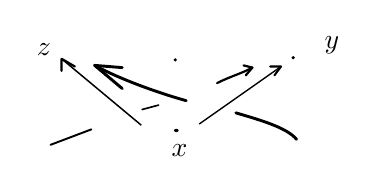
\begin{tikzpicture}[x=.014cm,y=-.014cm,line cap=round,line join=round]
\node at (31,35) {$z$};
\node at (292,31) {$y$};
\node at (154,126) {$x$};
\fill (150,44) circle[radius=.65pt];
\fill (257,42) circle[radius=.65pt];
\fill (151,108) ellipse[x radius=.85pt,y radius=.6pt];
\draw[line width=.55pt] (119,103) -- (47,43);
\draw[line width=.8pt] (47,54) -- (47,43) -- (59,50);
\draw[line width=.5pt] (172,102) -- (246,50);
\draw[line width=.75pt] (236,50) -- (246,50) -- (240,58);
\draw[line width=1.05pt] (160,81) .. controls (135,74) and (101,62) .. (77,49);
\draw[line width=1.05pt] (102,51) -- (77,49) -- (102,70);
\draw[line width=.8pt] (188,65) .. controls (200,59) and (211,56) .. (220,51);
\draw[line width=.8pt] (212,49) -- (220,51) -- (214,58);
\draw[line width=.7pt] (37,121) -- (74,107);
\draw[line width=.6pt] (120,89) -- (135,85);
\draw[line width=1.05pt] (205,92) .. controls (225,98) and (251,105) .. (260,116);
\end{tikzpicture}}
\end{minipage}\hfill\begin{minipage}[c]{.63\linewidth}
[On note que $y$ et $z$ sont non congrus mod $\sigma$, à cause de 28 a),]
\end{minipage}

Si $\unsure{\deleted{x}}y$ et $\unsure{\deleted{y}}z$ étaient incomparables; on aurait que $\sigma y$ et $z$ sont comparables, On \unsure{peu|pas|ne} peut avoir $z\leq\sigma y$ car on. aurait $x\leq\sigma y$, ce qui contredit $x<y$ par (28) a). On \deleted{\unsure{ne peut avoir}} \inserted{aurait donc} $\sigma y<z$ d'où $\sigma z<\unsure{\backslash|x}$

\clearpage

\scanpage{41}
\begin{flushright}
\unsure{relations|relatons} d'\unsure{èquiv.|equiv.|équiv.|èqui.|equi.}\hspace*{.8em}\\
non \unsure{panachées|panachés}
\end{flushright}

% archive sheet number: 40

\clearpage

\scanpage{42}
Soit $S$ un ens fini \inserted{Cardinal\unsure{,} $N$}, avec une structure \unsure{polygonale|polygonal} ou \unsure{bi-circularisation|bi-circulation} $\{u,u^{-1}\}$ ($\mathrm{Card}\,S\geq\unsure{3|2}$).\unsure{,}

\deleted{\uline{\unsure{Ax|Ax.|Déf.}}} $T\subset S$ \inserted{de cardinal $i$} est dit un \deleted{\unsure{ens}} \uline{segment} de $S$, si

a) \deleted{\unsure{non|on}} $T\ne S$, $T\ne\varnothing$ \deleted{$i<N$} i.e. $0<i<N$

b) $\exists\,\unsure{s|E}_0\in S$, \deleted{$i\in\unsure{\mathbb N|N}$}, tel que $T=\{s_0,us_0,\ldots,u^{i-1}s_0\}$

(donc, posant $t_0={\unsure{w|u}}^{i-1}s_0$, on aura aussi $T=\{t_0,vt_0,\ldots,v^{i-1}t_0\}$, où $v=u^{-1}$).

\uline{Ex.} les parties réduites : un point.

les \unsure{parties-arêtes}\unsure{.}

\margin{\deleted{\uline{\unsure{Propr.|Prop.}} \unsure{Soit|Soient} $A\unsure{,}A'$ deux \unsure{segments},}}

$T$ est un segm. \unsure{sss|ssi} $S\setminus T$ en est un.

\inserted{Intersection de deux segments \inserted{\unsure{\uuline{contenus dans un segment}|\uline{contenus dans un segment}|contenus dans un segment}} \unsure{(}en est un sss il est $\ne\varnothing$\unsure{)}}

\inserted{Réunion de deux segments \unsure{pris ds un contexte|pris ds un contre-ex.|qui se rencontrent}, et tels que $T'\cup T''\ne S$ \inserted{est un segment}}

\margin{\unsure{i.e|i.e.} de \unsure{\deleted{réunion}|réunion} $\ne S$}

Extrémités d'un segment $s_0,t_0$ (\unsure{distinctes} sss $i\ne1$ i.e. $T$ non réduit à un point).

Origine, extrémité pour une . orientation.

[ \uline{NB} Si $u$ i.e. l'orientation choisi, le $s_0$ est unique i.e. il y a corr. \unsure{1-1|11} entre l'ens des segments de $S$, et l'ens
\[
 (S,[1,N-1]_{\mathbb N}),\ \text{via}\quad (s_0,i)\longmapsto\{s_0,us_0,\ldots \underset{\unsure{\cdot\!{}^{\cdot}}}{u}^{i-1}s_0\}.
\]

\unsure{\deleted{P|S}}Soit $S'\subsetneq S$ une partie de $S$. Alors \deleted{les segments de $S$ contenus} deux segments de $S'$ contenus ds $S'$, et qui se rencontrent, ont comme réunion un segment \inserted{de $S$} contenu dans $S'$ -- \unsure{cel|cela} implique
% archive sheet number: 41

\clearpage

